
%(BEGIN_QUESTION)
% Copyright 2014, Tony R. Kuphaldt, released under the Creative Commons Attribution License (v 1.0)
% This means you may do almost anything with this work of mine, so long as you give me proper credit

En {\bf resistiv tape}-nivåsensor er et tolederelement nedsenket i væske, der resistansen endres når nivået øker. Prinsippet ligner å sette foten med gummistøvel ned i vann: jo dypere foten er nedsenket, desto lengre opp på fot og ankel kjenner du at vanntrykket presser støvelen mot huden. En resistiv tape går over hele tankhøyden, og kontakt mellom to resistive ledere oppstår ved hydrostatisk trykk over den nedsenkede delen av tapen. Jo høyere væskenivå, desto lengre del av lederne er i kontakt, og dermed blir total resistans lavere.

Studer følgende resistive tape-målesystem og beregn følgende, gitt maksimal taperesistans 10 k$\Omega$ (dvs. uten nedsenking), minimal resistans 2 k$\Omega$ (dvs. full nedsenking), lineær sammenheng mellom nedsenking og resistans, og total tapelengde 15 fot:

$$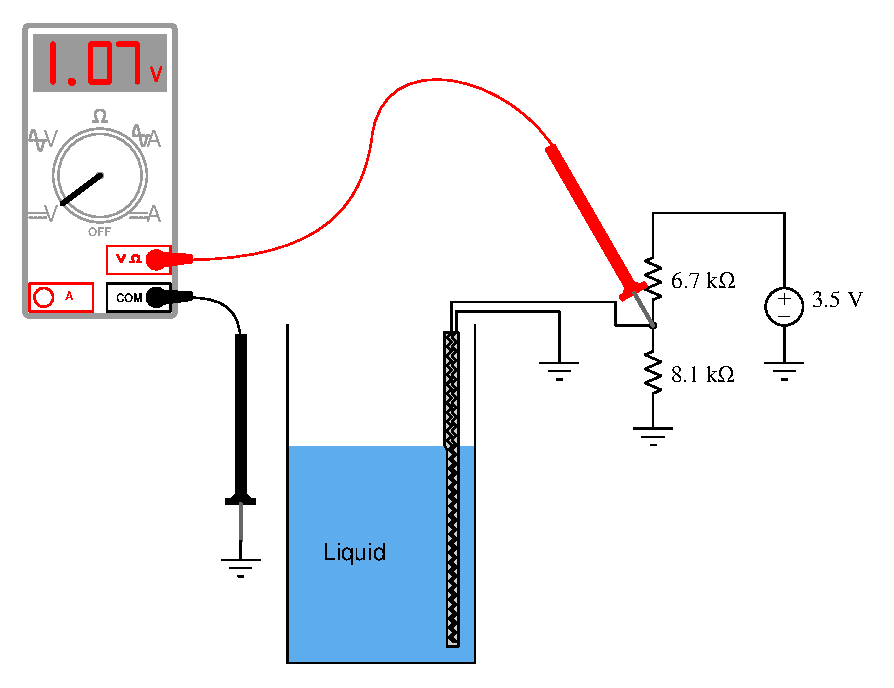
\includegraphics[width=15.5cm]{i00855x01.eps}$$

Tape-resistans ($R_{tape}$) = \underbar{\hskip 50pt}

\vskip 10pt

Nedsenkingsdybde = \underbar{\hskip 50pt}

\vfil 

\underbar{file i00855}
\eject
%(END_QUESTION)





%(BEGIN_ANSWER)

Dette er en vurdert oppgave -- ingen svar eller hint oppgis!

%(END_ANSWER)





%(BEGIN_NOTES)

Først må vi bestemme taperesistansen. Her er det nyttig å tegne en ekvivalent krets:

$$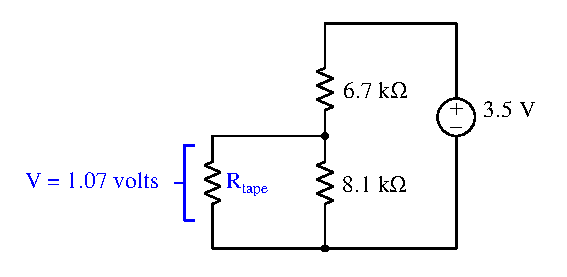
\includegraphics[width=15.5cm]{i00855x02.eps}$$

Når tapen har 1.07 V spenningsfall, må 6.7 k$\Omega$-motstanden ha resten opp til 3.5 V (kildespenning):

$$V_{6.7k} = 3.5 \hbox{ V} - 1.07 \hbox{ V} = 2.43 \hbox{ V}$$

Dette lar oss beregne total kretsstrøm, siden all strøm går gjennom 6.7 k$\Omega$-motstanden:

$$I = {V \over R} = {2.43 \hbox{ V} \over 6700 \> \Omega} = 0.363 \hbox{ mA}$$

Strømmen 0.363 mA fordeler seg når den kommer til parallellgrenene med resistiv tape og 8.1 k$\Omega$-motstanden. Vi finner tapestrømmen ved å beregne strømmen gjennom 8.1 k$\Omega$ og trekke den fra totalen 0.363 mA (Kirchhoffs strømlov). Først strømmen i 8.1 k$\Omega$:

$$I = {V \over R} = {1.07 \hbox{ V} \over 8100 \> \Omega} = 0.132 \hbox{ mA}$$

Bruker KCL for tapestrøm:

$$I_{tape} = 0.363 \hbox{ mA} - 0.132 \hbox{ mA} = 0.231 \hbox{ mA}$$

Nå kjenner vi tapestrøm (0.231 mA) og tapespenning (1.07 V), og kan beregne motstanden:

$$R = {V \over I} = {1.07 \hbox{ V} \over 0.231 \hbox{ mA}} = 4640.3 \> \Omega$$

\vskip 10pt

\filbreak

Beregn nedsenkingsdybde med lineær funksjon. Vi vet at tapen har 10 k$\Omega$ når den er tørr (0 fot nedsenking) og 2 k$\Omega$ ved full nedsenking (15 fot). Vi lager en lineær funksjon mellom nedsenkingsdybde og resistans, og setter inn kjent resistans 4.6403 k$\Omega$ for å finne dybden:

$$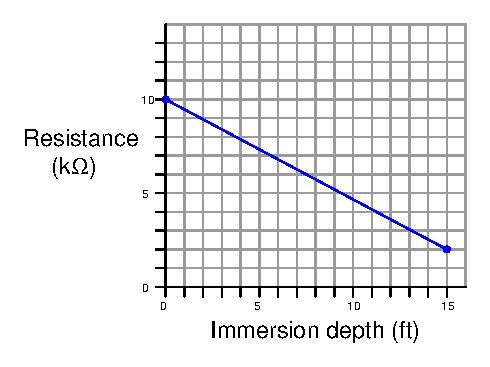
\includegraphics[width=15.5cm]{i00855x03.eps}$$

Standardformel for lineær funksjon:

$$y = mx + b$$

\vskip 10pt

Stigningstall ($m$):

$$m = \hbox{slope} = {\hbox{rise} \over \hbox{run}} = {2 - 10 \over 0 - 15} = - {8 \over 15}$$

\vskip 10pt

Setter stigningstall inn i $y = mx + b$:

$$y = -{8 \over 15}x + b$$

\vskip 10pt

Finner konstantledd ($b$) ved å bruke et kjent punkt, for eksempel $x=0$, $y=10$:

$$10 = -\left({8 \over 15} \right) 0 + b$$

$$b = 10$$

\vskip 10pt

Endelig funksjon:

$$y = -{8 \over 15}x + 10$$

\vskip 10pt

\filbreak

Sett inn kjent resistans og løs for nedsenking. Merk at funksjonen bruker resistans i {\it kilo}-ohm, så vi bruker 4.6403 og ikke 4640.3:

$$4.6403 = -{8 \over 15}x + 10$$

$$-5.3587 = -{8 \over 15}x$$

$$x = 10.049$$

Dermed er tapen nedsenket i 10.049 fot væske.






%INDEX% Measurement, level: hydrostatic pressure

%(END_NOTES)
